\documentclass{article}

\usepackage[utf8]{inputenc}
\usepackage{graphicx}
\usepackage{amssymb}
\usepackage{amsmath}

\title{Assignment 1}
\author{Gollapudi Sasank CS21BTECH11019}
\date{30 March 2022}

\begin{document}

\maketitle
\section*{ICSE 2018 Question 6 (a)}
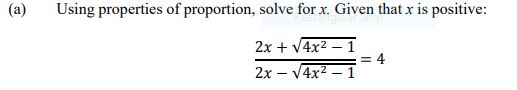
\includegraphics[width=\columnwidth]{Question.png}
From the properties of proportion \\ 
\begin{equation*}
     \frac{a}{b}  =  \frac{c}{d} 
     \Rightarrow 
     \frac{a+b}{a-b} = \frac{c+d}{c-d} \hspace{40pt} -(1) \\
\end{equation*}
The Given Equation is :
    \begin{equation*}
    \centering
        \frac{2x+\sqrt{4x^2-1}}{2x-\sqrt{4x^2-1}} = \frac {4}{1}
    \end{equation*}
    From (1) 
\begin{equation*}
        \frac {2x+\sqrt{4x^2-1}+2x-\sqrt{4x^2-1}}{2x+\sqrt{4x^2-1}-2x+\sqrt{4x^2-1}} = \frac {4+1}{4-1} \\
\end{equation*}
\begin{equation*}
        \Rightarrow
        \frac{4x}{2\sqrt{4x^2-1}} = \frac {5}{3} \\
\end{equation*}
\begin{equation*}
        \Rightarrow
        \frac{6x}{5} = \sqrt{4x^2-1} \\
\end{equation*}
\begin{equation*}
    \Rightarrow
        \frac{36x^2}{25} = 4x^2-1 \\
\end{equation*}
\begin{equation*}
        \Rightarrow
        1 = (4 - \frac{36}{25} )  x^2 \\
\end{equation*}
\begin{equation*}
    \Rightarrow
    x^2 =\frac{25}{64} \\ 
\end{equation*}
\begin{equation*}
    \Rightarrow
    x = \pm\frac{5}{8} \\
\end{equation*}
But Given x is positive 
\begin{equation*}
  \Rightarrow x = \frac{5}{8} \\  
\end{equation*}
\end{document}
